%----------------------------------------------------------------------------
\chapter{\bevezetes}
%----------------------------------------------------------------------------
Nowadays the usage of a multi-layered applications have increased, however these can be very complex systems. They are often used in a safety-critical environment, therefore the need to create a reliable application is important. In this area a software or hardware failure can cause unsafe events with high risks. In addition finding a problem's root cause can be time-taking in the latter development phases. To avoid such a situation the most common verification method is testing. Several failures and errors can be found by a detailed and well-designed testing framework.

The need for a maintainable testing structure have also came up in the department of Measurement and Information Systems for a safety-critical project. The Model-based Demonstrator for Smart and Safety Systems (in abbreviation: MoDeS$^3$) relies on a model railway system and have been extended with hardware and software elements to control the track and trains on it. Its purpose is also to demonstrate the model-based design and verification techniques. To satisfy these objectives, off-the-shelf and custom hardware elements have been attached to the railway track. These products required also custom-made software components, which have several technological dependencies making the demonstrator system a complex multi-layered application. The track consists of 24 sections and 6 turnouts, for which 6 BeagleBone Black microcontrollers have been configured with custom hardware extensions to control them. An Arduino microcontroller have been added to the system to sense the availability (shows that for example a train is on a segment or not) of each segment In addition a Raspberry PI provides a graphical interface to control the track elements separately and supplies the necessary technical environment for the other microcontrollers. A picture of the whole track is shown in \autoref{fig:overview} from top view.

\begin{figure}[ht]
	\centering
	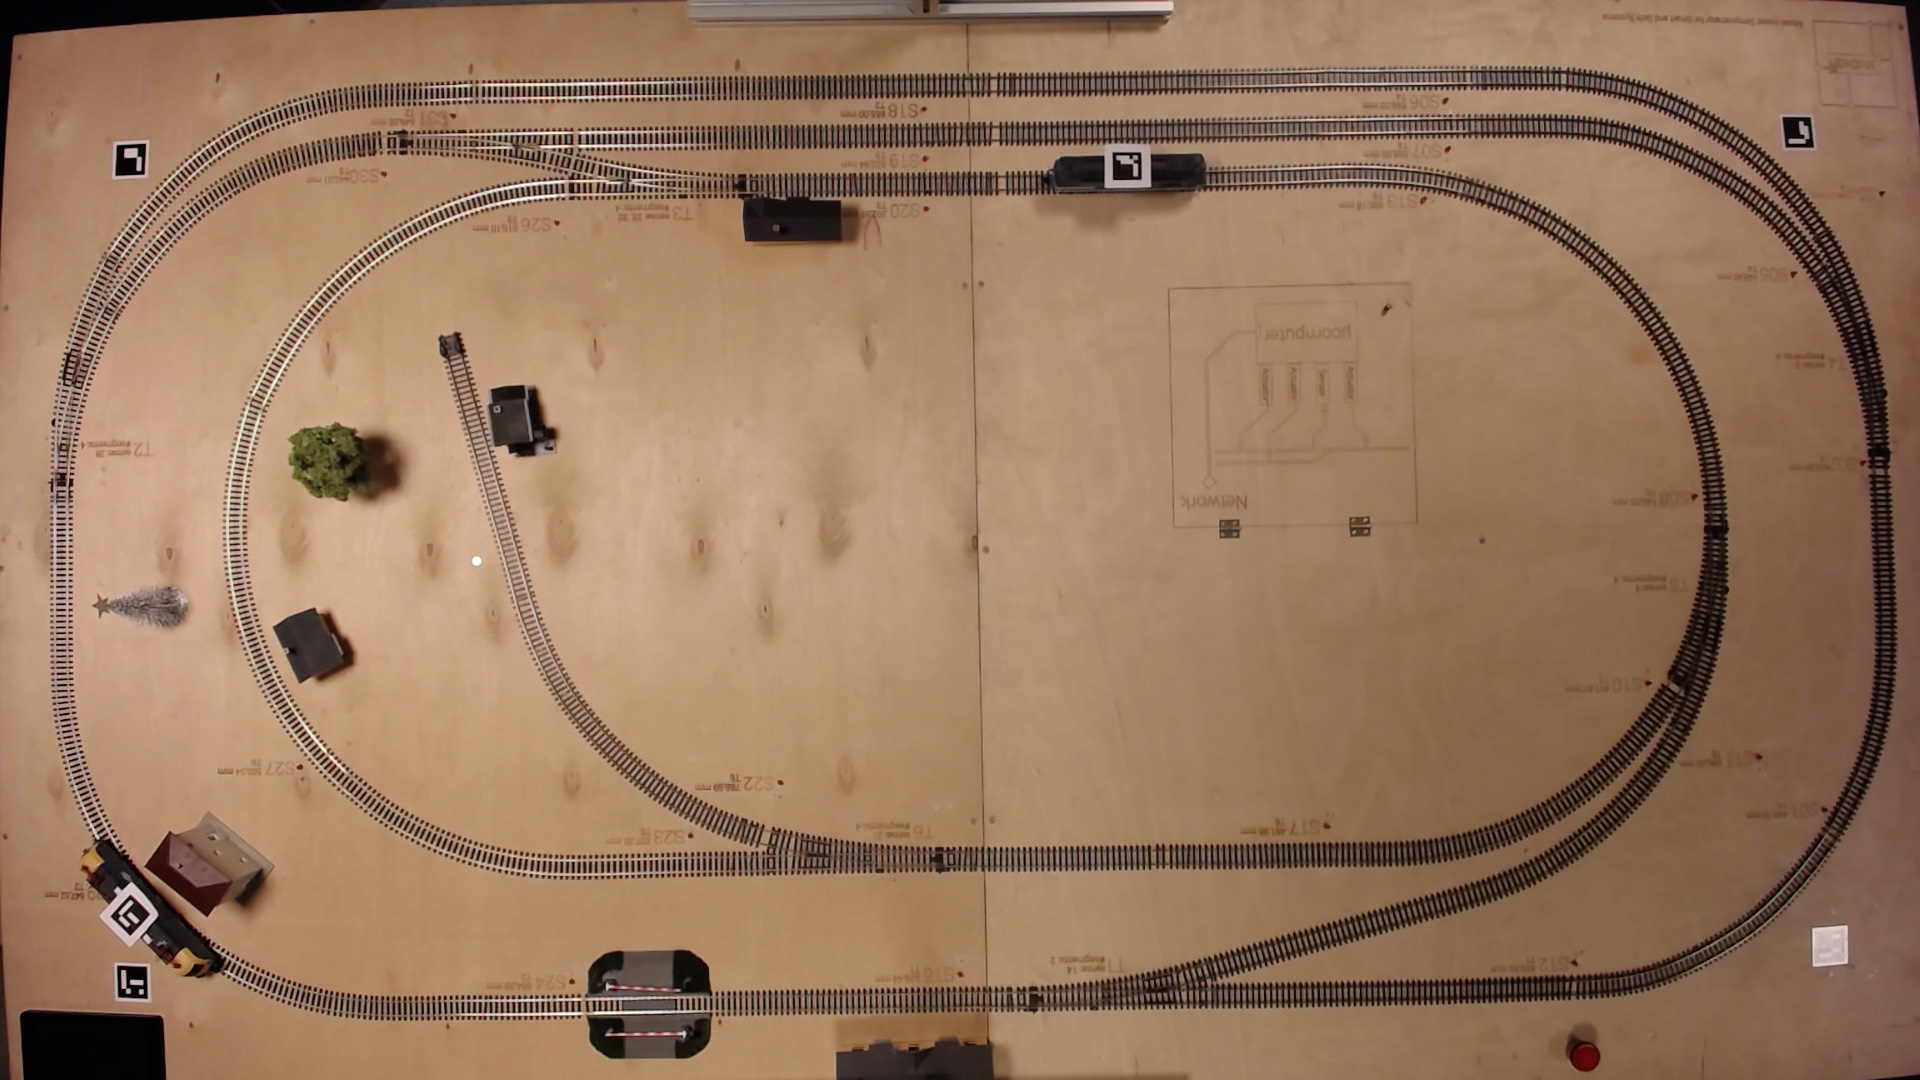
\includegraphics[width=150mm, keepaspectratio, angle = 180]{figures/modes3/overview.jpg}
	\caption{Railway system top overview}
	\label{fig:overview}
\end{figure}

During the development of MoDeS$^3$ system, there wasn't a maintainable and well-designed testing approach, which is able to follow the frequently changing software and hardware implementations. Right now the demonstrator system basic functionalities become more stable, but the need for a testing framework is still remained. In my thesis I will investigate the possible test approaches for creating a suitable test environment for the railway system. In order to construct a maintainable and applicable test framework for the system, all parts must be examined which we are aiming to test. The first aspect is to detail and verify the safety-critical functionalities with requirements. Then a systematic and detailed test design can be created for the project.

To start with I have defined the requirement for the demonstrator system and detailed the safety-critical aspects, which should be covered by tests. A systematic and detailed test design have been constructed for testing purposes aligned with the ISO 29119 standard \cite{IEEE13}. This documentation was helpful for creating a maintainable and systematic test documentation for such a complex system. The MoDeS$^3$ demonstrator railway system requires a wide knowledge in the model driven and low level (close to hardware) technologies also. On the microcontrollers Java executables are deployed, except the Arudino component for which a C++ unit is installed. Therefore the test plans have to be designed to support implementations in multiple languages. Additionally high-level model-based techniques are used to avoid safety-critical situations on the track, like Viatra, Yakindu with Gamma, which can generate Java classes representing their models. Throughout the implementation, Eclipse was used with Xtend plugin, which generates the source code into Java classes. Therefore I have used the JUnit 5 library along with Mockito and PowerMock frameworks for test case implementation.

In my thesis I describe the architecture of the MoDeS$^3$ railway demonstrator system in \autoref{chapter:RailwaySystem}, where after the custom hardware and software components, the safety-critical scenarios and functions are detailed, aligned with the system requirements. In the next \autoref{chapter:TestDoc}, the possible test design techniques are detailed with the overview of the test documentation standard. After the description of system architecture and the general test documentation chapters, the \autoref{TestDoc:MODES} follows with the design decisions and details of the test documentation for MoDeS$^3$ system. The test implementation key points and the status of test execution reports are described in \autoref{TestImpl:MODES}. Finally the \autoref{chapter:Summary} summarizes my thesis work.

